% !TeX spellcheck = it_IT
\chapter{Introduzione}
\chapter{Cenni biografici}
Paul Bley nacque a Montreal, in Canada, il 10 Novembre 1932. I genitori adottivi furono Betty Marcovitch, emigrata rumena di modeste origini, e il facoltoso imprenditore tessile Joe Bley\footcite[10]{stopping}. Paul era in verità figlio biologico di Joe e di una sua dipendente (una donna del Canada francese di nome Lucie): dal momento che Betty non poteva avere figli, Bley fece mettere il neonato in orfanotrofio per convincere poi la moglie, ignara della situazione, ad adottarlo; la madre biologica di Paul venne poi assunta come balia dalla famiglia. Lo stesso Paul non sarebbe venuto a conoscenza di questo fatto fino a molti anni dopo, nel 1992\footcite[13]{stopping}. La madre adottiva, in ogni caso, crebbe il bambino con affetto e cura, decidendo di impartirgli un'educazione musicale e di fargli frequentare la scuola della comunità ebraica di Montreal.\\
La rivelazione del fatto di essere stato adottato (nonostante entrambi i genitori biologici fossero in realtà presenti) fu un evento traumatico per il bambino, spingendolo a rifugiarsi nella musica per colmare la mancanza di un senso di appartenenza. Il divorzio dei genitori aggiunse ulteriore stress sul giovane Paul, che ricorda come in quegli anni (anche grazie al suo insegnante August Dècarie) maturò in lui la decisione di diventare un musicista professionista\footcite[15]{stopping}. Sempre in quel periodo Paul ebbe il suo primo contatto con il concetto di improvvisazione:
\begin{fquote}
	Oltre alla scuola, stavo iniziando a studiare per il mio Bar Mitzvah, per il quale avrei dovuto cantare un testo in ebraico. Quando chiesi al mio rabbino ``Come fa la melodia?'' egli rispose ``Inventala sul momento''.
	\end{fquote}
\appendix
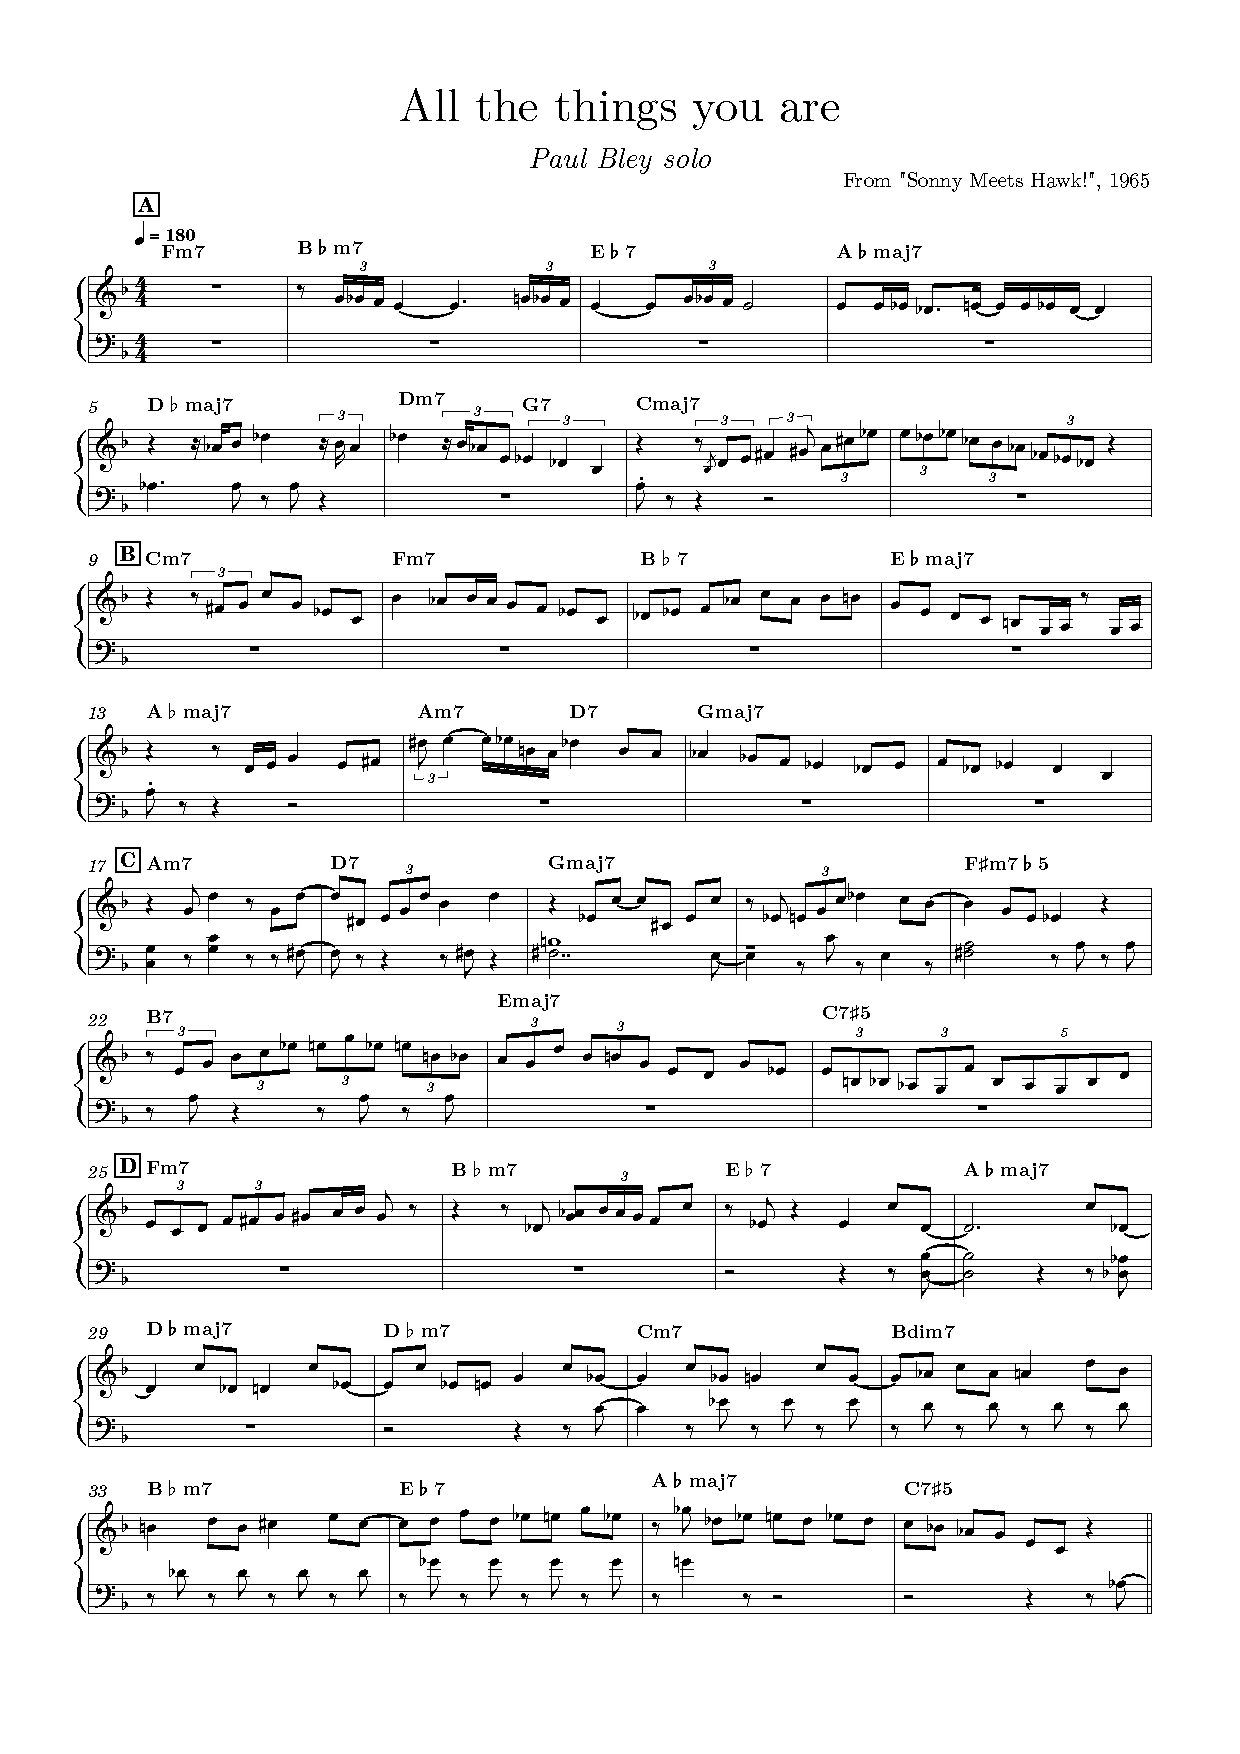
\includepdf[pages=-,pagecommand={},scale=0.9]{things_vanilla}